\section{Scalable RF Clock Synchronization}
\label{sec_iris_clocking}

	Stable, low-noise, and synchronized clocking is necessary for a coherent \ac{MIMO} array.
	For example, when a noisy reference clock is used for \ac{ADC} or \ac{DAC} sampling clocks it results in \textit{aperature uncertainty} error \cite{brannon2006jitter} by causing the system to sample at non-ideal and randomly-varying time intervals.
	When the noisy reference clock is used as a reference for carrier synthesis, it manifests as \textit{phase noise} in the input and output RF signal \cite{an687}.
	
	In addition to the noise caused by RF reference clock jitter, additional transceiver impairments such as carrier frequency offset of the radio's frequency mixer circuits and sample frequency offset of the radio's \acp{ADC} rapidly degrades the performance of \ac{ZFBF} in even small $4\times 4$ systems \cite{rogalin2014scalable}.
		Theoretical studies of many-antenna systems in the presence of phase noise have shown that this noise source can result in well over 50\% or more decrease in sum throughput in both the many-antenna uplink \cite{krishnan2014impact} and downlink \cite{pitarokoilis2012effect} systems.
	As \ac{MIMO} systems increase in size, the generation and distribution of a reference clock becomes a more difficult system-level design challenge whether for a single co-located array of radios or in a distributed \ac{MIMO} system such as those proposed for 5G cellular \cite{cui2014evolution, ali2014evolution}.
	
	In this section, we present the design and evaluation of a number of different practical clocking topologies in large-scale coherent \ac{SDR} systems, presenting new measurement results of unique clocking topologies that we have implemented.
	Based on our insight gained from developing the $8\times 8$ \ac{WURC} \ac{SDR} in Section~\ref{sec_wurc_8x8} we present a novel daisy-chained clocking architecture for next-generation systems that increases the number of radios while reducing the amount of cabling required compared to other large-scale \ac{MU-MIMO} systems.
	Consequently, reliability and portability is improved.
	
	Another consideration for large-scale \ac{TVWS} systems is that the large size of antennas spaced at a half-wavelength for spatial diversity will need to be addressed.
	We develop a robust, distributed, and low-cost system for distributing an RF reference clock with a daisy-chain radio topology as a new approach to solving this challenge.
	An added benefit is that the modularity of the design yields freedom when considering the physical configuration of the radios and can enable new experiments in distributed \ac{MIMO}, \ac{CoMP}, and other coherent radio technologies at very large scale.

%\rgnote{This section is the new work I've done on the Iris platform that Dr. Zhong asked for and is beign finalized right now. A discussion regarding clock synchronization techniques, GPS timing synchronization and how it is not appropriate for coherent CoMP (seriously, literally everyone I talk to about CoMP brings this up incorrectly), and a measurement study of our innovative clock regeneration scheme for Iris that ensures essentially unlimited clock domain scaling and absolute deployment flexibility vs. all other approaches I've seen to date. This section builds on the concept in sections, presenting the clocking structure design and evaluation for WURC, WURC Array, IRIS, then finally Faros as the evolution of scalable clocking.}



%###############################################
\subsection{Cooperative Multi-Point and Network \ac{MIMO}}
\label{sec_comp_brief}

% Table generated by Excel2LaTeX from sheet 'Sheet1'
\begin{table}[h]
  \centering
  \caption{Comparison of CoMP Techniques and Required System Support.}
  \resizebox{1\textwidth}{!}{%
    \begin{tabular}{llllll}
          & \multicolumn{5}{c}{\textbf{Coordinated Multi-Point (CoMP)}} \\
\cmidrule{2-6}          & \multicolumn{2}{c}{\textbf{Coordinated Switching/Beamforming (CS/BF)}} & \multicolumn{3}{c}{\textbf{Joint Processing (JP)}} \\
\cmidrule{2-6}          & \multicolumn{1}{c}{\multirow{2}[2]{*}{\textbf{Coordinated Beam-Switching (CBS)}}} & \multicolumn{1}{c}{\multirow{2}[2]{*}{\textbf{Coordinated Switching (CS)}}} & \multicolumn{2}{p{12.64em}}{\textbf{Joint Transmission (JT)}} & \multicolumn{1}{c}{\multirow{2}[2]{*}{\textbf{Dynamic Point Selection (DPS)}}} \\
          &       &       & \multicolumn{1}{c}{\textbf{Coherent}} & \multicolumn{1}{c}{\textbf{Non-Coherent}} &  \\
    \midrule
    \midrule
    \textbf{User Data Location} & One BTS & One BTS & All   & All   & All \\
    \textbf{Pre-coding Decision} & Individual & Individual & Joint & Individual & Individual \\
    \textbf{Timing Sync Needed} & \cellcolor[rgb]{ .922,  .945,  .871}Yes & \cellcolor[rgb]{ .922,  .945,  .871}Yes & \cellcolor[rgb]{ .922,  .945,  .871}Yes & \cellcolor[rgb]{ .922,  .945,  .871}Yes & \cellcolor[rgb]{ .922,  .945,  .871}Yes \\
    \textbf{Clock Sync Needed} & \cellcolor[rgb]{ .949,  .863,  .859}No & \cellcolor[rgb]{ .949,  .863,  .859}No & \cellcolor[rgb]{ .922,  .945,  .871}Yes & \cellcolor[rgb]{ .949,  .863,  .859}No & \cellcolor[rgb]{ .949,  .863,  .859}No \\
    \end{tabular}%
	}
  \label{tab_comp_types}%
\end{table}%


	\ac{CoMP} typically refers to multi-cell transmit coordination \cite{ali2014evolution} for improving user signal strength or mitigating inter-cell interference.
	However, taken to its limit, a logically modular, coherent, and distributed \ac{MIMO} system may not have a clear concept of a ``cell.''
	For example: clusters of coherent \ac{WURC} radios could be distributed across a rooftop or across an office ceiling to provide ubiquitous coverage and large array aperature size.
	For the purpose of this discussion, we will define \ac{CoMP} as the simultaneous use of transmitters that are physically located much further than a single wavelength apart in order to increase signal strength and reduce interference in a wireless network.
		
	There are many different types of inter-cell or inter-\ac{AP} coordination, each with their sets of system requirements and tradeoffs.
	We present an overview of \ac{CoMP} techniques in Table~\ref{tab_comp_types} corresponding to the taxonomy proposed by Ali et. al. \cite{ali2014evolution} in order to clarify our target system design; for more details regarding these techniques, we direct the reader to the references therein.
	Other work has shown that while the system burden can be quite high, the performance of coherent \ac{JT}-\ac{CoMP} consistently outperforms other techniques for users at the cell edge \cite{cui2014evolution, kim2017call}, and is one of the few techniques that increases network spectral efficiency, making it very desirable for next-generation networks.
	
	We focus on delivering a scalable, physical layer clock synchronization solution that enables coherent \ac{JT}-\ac{CoMP} or, equivalently, ``network \ac{MIMO}'' \cite{huh2012network}.
	
		At this point, it is useful to define a few terms that will be useful for this discussion.
	Relative clock \textbf{skew} is the time difference between two clocks as defined by their edge, or the relative point in time when two clock signals cross a voltage threshold.
	Clock \textbf{jitter} is the short-term variation in clock frequency, often empirically measured as the \ac{TIE}, or the distribution of error between the actual clock edge and an ideal clock edge over a large sample size.
	Clock \textbf{wander} is the long-term variation in clock frequency, sometimes characterized as frequency dynamics occuring below 10~Hz.
	Finally, we will use the term \textbf{syntonized} to refer to two clocks that have the same oscillation frequency, but may each have arbitrary phase relative to each other; once those two clocks share absolute phase (or have information regarding the offset such that it can be removed or ignored), then they are considered \textbf{synchronized}.
	
%###############################################
\subsection{Alternative Distributed Clocking Architectures}
\label{sec_comp_alts}

\textbf{Massive MIMO Clocking.}
	Several Massive \ac{MIMO} testbeds have been constructed from \ac{NI} hardware using the \ac{NI} CDA-2990 or ``OctoClock'' to form a two-tiered or radial clocking network with coaxial cables linking back to a grand master reference clock \cite{luther20145g}.
	Identical hardware and clocking topologies have been reported for the testbeds used by Lund and Bristol Universities \cite{vieira2014flexible}, as well as Facebook Project ARIES \cite{choubey2016introducing}.
	Previous generations of many-antenna systems at Rice University have also used a similar, flat clocking topology \cite{shepard2012argos, shepard2013argosv2}.
	Both timing and synchronization are accomplished via flat or tiered clock distribution buffers and each link requires a coaxial cable for both clock distribution and timing synchronization reference, resulting in large, bulky systems.
	
\textbf{GPS-Disciplined Oscillators.}
	Jungnickel et. al. report a carrier frequency offset of $6\cdot10^{-10}$ between two Rubidium GPS-conditioned oscillator platforms after 24 hours of outdoor signal conditioning \cite{jungnickel2008synchronization}.\footnote{It might be unintuitive at first glace, but \ac{GPSDO} platforms increase in precision over time as they integrate more timing observations from more \ac{GPS} satellites.}
	This corresponds to 0.6~ppb at their 10~MHz reference, or 3.12~ppb at 52~MHz, the reference frequency of our system's \ac{MEMS} oscillators with 100~ppb accuracy.
	The authors claim that syntonization between \ac{JT}-\ac{CoMP} points is not required since residual carrier offset can be tolerated.
	Nevertheless, their system only demonstrates a low-order $2\times 2$~\ac{ZFBF} and required a \ac{GPS} synchronization period of 24 hours before the \ac{GPS} oscillators had sufficient observations to avoid excessive noise with 5~ms of time between channel sounding and \ac{ZFBF} transmission.
	This represents a relatively easy demonstration case since longer transmission intervals with older \ac{CSI} would have required even lower carrier frequency offset than that demonstrated, and our system targets array sizes much larger than two radios which increases the performance requirements proportionally.
	With the inability to practically operate indoors or at large time scales between refreshing \ac{CSI}, we disagree with the author's conclusion that RF syntonization is not necessary for large-scale \ac{CoMP}.
	
\textbf{Over-the-Air Synchronization}
 Rogalin et. al. proposed an over-the-air frequency synchronization and offset compensation algorithm that allowed distributed \ac{MIMO} nodes to perform coherent operations \emph{without} syntonization; however the achievable rate degrades extremely rapidly due to clock drift over the course of \emph{milliseconds} in just a $4\times 4$ system (28\% loss of achievable rate over 16~ms, \cite{rogalin2014scalable}, Figure 5).

	For these reasons, we argue that syntonization is a system-level requirement for \ac{JT}-\ac{CoMP} with many radios and that \ac{GPS} and over-the-air techniques proposed in the literature are inadequate for large-scale distributed systems.
	
\textbf{White Rabbit.}
	The White Rabbit Project seeks to solve a similar distributed clock and timing synchronization problem.
	Custom networking hardware was developed for the \ac{CERN} Large Hadron Collider experiment and manufactured by Seven Solutions S.L., \cite{lipinski2011white, serrano2013white} utilizing a Layer 1 Synchronous Ethernet (Sync-E) switching network \cite{rec2007g} for syntonization, the IEEE1588 \ac{PTP} protocol for coarse synchronization, and a custom \ac{DDMTD} algorithm to fine-tune clock phase offsets in order to produce distributed clock synchronization with sub-ns accuracy \cite{wlostowski2011precise}.

In our solution, we seek to remove the hardware complexity, cost, and deployment restrictions of large-scale radial or tiered clock distribution topologies while achieving the high-precision syntonization among a distributed set of coherent radios achievable with White Rabbit.
	Our key observation is that unlike the White Rabbit solution, coherent \ac{CoMP} requires only syntonization, provided all timing events are deterministic without variable delay exceeding some threshold.
	For instance, there are significant provisions within White Rabbit to compensate for the light propagation delay for uplink vs. downlink fiber lasers that are not necessary in a system-level design of a \ac{JT}-\ac{CoMP} radio access network.
	
	This relaxation of our \ac{CoMP} system requirements compared to those of the Large Hadron Collider results in the ability to design a distributed, high-precision clocking architecture that utilizes a commodity Layer 1 synchronous fiber-channel Ethernet backplane.
	This design can be implemented with little additional hardware components on the distributed radio heads compared to White Rabbit hardware implementations.
	A benefit of this system design choice, shared with White Rabbit, is that \ac{JT}-\ac{CoMP} requires user data to be distributed to the cooperating base stations anyway, so re-using the existing data backplane for high-precision clock distribution is ideal.

\pagebreak

%###############################################
\subsection{Tiered Modular Clock Synchronization}
\label{sec_tiered_clocking}

%\rgnote{Tiered clocking: what I did for WURC and 4x1 WURC with a flat clocking hierarchy}

Since the transmit and receive chains in a \ac{MU-MIMO} base station require precise phase synchronization, \ac{WURC} was designed to draw RF reference clocks from the host digital baseband board as shown in Fig.~\ref{fig:wurc_clock_diagram}.
This simplifies the digital design since both the \acp{DAC} and \acp{ADC} are driven with the same clock as the rest of the digital signal processing path in the \ac{FPGA}.

%\rgnote{Discussion of FPGA and native clocking jitter and the evolution of the adaptor design based on iterative measurements and testing.} 

\begin{figure}[h]
\centering
  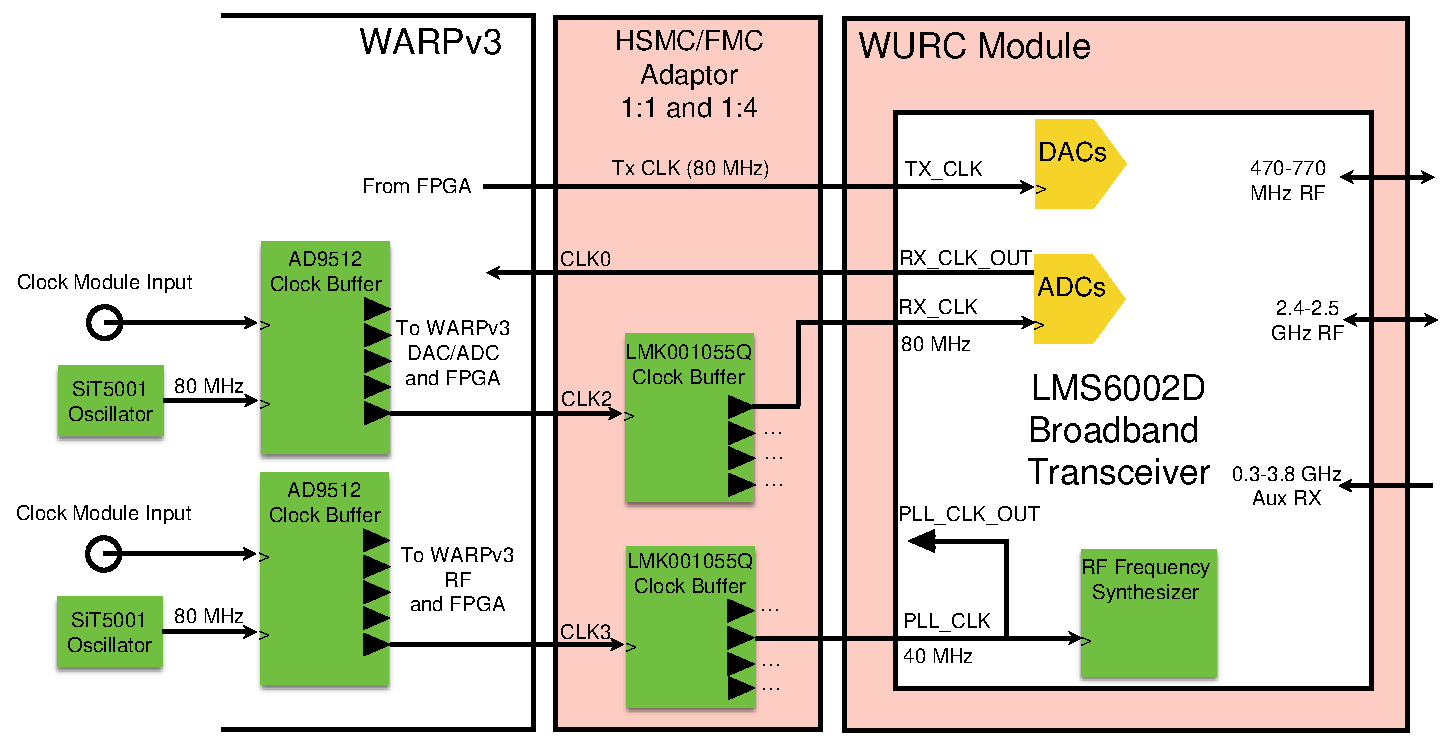
\includegraphics[width=4.5in]{figs/clk/wurc_clock_diagram_2}   
    \caption{Source-synchronous sampling clocks and RF reference clocks are buffered in stages, permitting fanout to up to 4 radios.}
\label{fig:wurc_clock_diagram}
\end{figure}

We placed an additional RF reference and sampling clock buffer, a Texas Instruments LMK001055, on the FMC/HSMC adapter rather than on the daughtercard itself so that the designed system can scale up to four \ac{WURC}s driven from a single host FPGA with synchronized clocks.
A single forwarded clock branch is used in the 1:1 HSMC/FMC adaptor shown in Figure~\ref{fig_warp_wurc_hw}, however the full 4 branches of clock buffering available in the design was used in the 4:1 HSMC/FMC adaptor used in the $4\times 4$ and $8\times 8$ \ac{WURC} arrays shown in Figures~\ref{fig:wurc_argos_hw} and \ref{fig:mimohw}.

Multi-tiered clocking trees have been proven out in the literature, in industry, and in our first \ac{WURC} \ac{SDR} platform as a reliable and manageable way to create coherent multi
Nevertheless, when we consider the task of delivering a single reference clock to potentially hundreds of discrete radios, the tiered topology quickly becomes unwieldy.
In the following section, we evaluate a new clocking architecture that addresses these concerns using next-generation \ac{SDR} hardware. 



%###############################################
\subsection{Multi-Hop Clock Synchronization}
\label{sec_daisy_chain_clocking}
	
In this section, we present the design and evaluation of a key architectural innovation required to scale our $8\times 8$ \ac{WURC}-array by an order of magnitude to 100s of radios that we designed and implemented on a new generation of commercial \ac{SDR} hardware.
	This newer ``IRIS-020'' and ``IRIS-030'' \ac{SDR} radio hardware is informed by our experience implementing the \ac{WURC} radio arrays, but for the sake of brevity, we will omit most of the system design since it architecturally mirrors that of \ac{WURC}.
	Instead, we will focus in this section on the design of IRIS's new many-radio clocking architectures as the primary research contribution of this new platform.

	An important feature of the IRIS \ac{SDR} hardware design is the ability to provide reference clock synchronization to a very large chain of Iris modules in order to act as a single, coherent array.
	In such an array, ensuring the integrity and accuracy of the RF reference clock is extremely important, since reference clock jitter manifests as noise in the digitized signal, potentially limiting system performance \cite{brannon2006jitter}.
	
	The design goal for the IRIS-020 system shown in Figure~\ref{fig_iris_pictures} (left) was to achieve a forwarded clock phase jitter less than 3~ps RMS given the initial system design parameters of 40~MHz modulation bandwidth and \ac{ADC} resolution of 10 bits \cite{brannon2006jitter}.
	This prototype \ac{SDR} module utilized a daisy-chained clock fanout buffer topology that buffered the reference clock signal at each intermediate node before forwarding to the next node (Figure~\ref{fig_020_chain})
	
% Daisy Chain Clocking Diagram- 020
\begin{figure}[p]
\centering
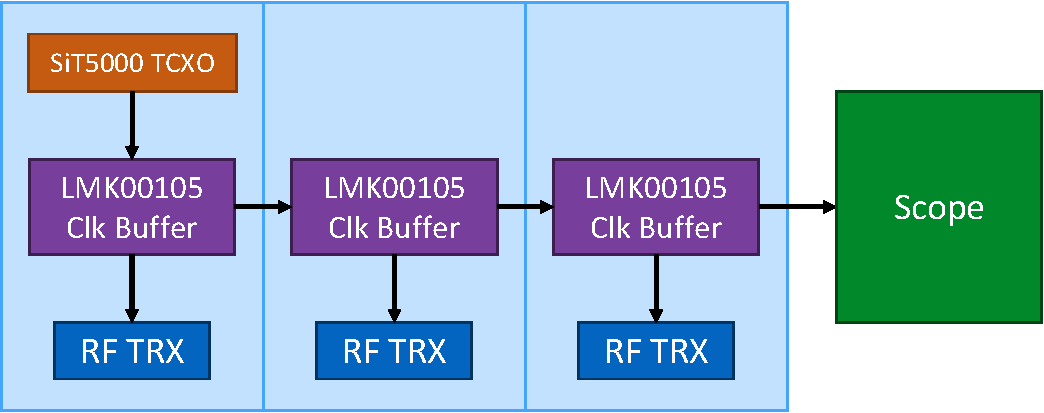
\includegraphics[width=0.7\textwidth]{figs/clk/iris020_diagram}
\caption{Block diagram of IRIS-020 buffered daisy chain clocks.}
\label{fig_020_chain}
\end{figure}

% Daisy Chain Clocking Diagram -030
\begin{figure}[p]
\centering
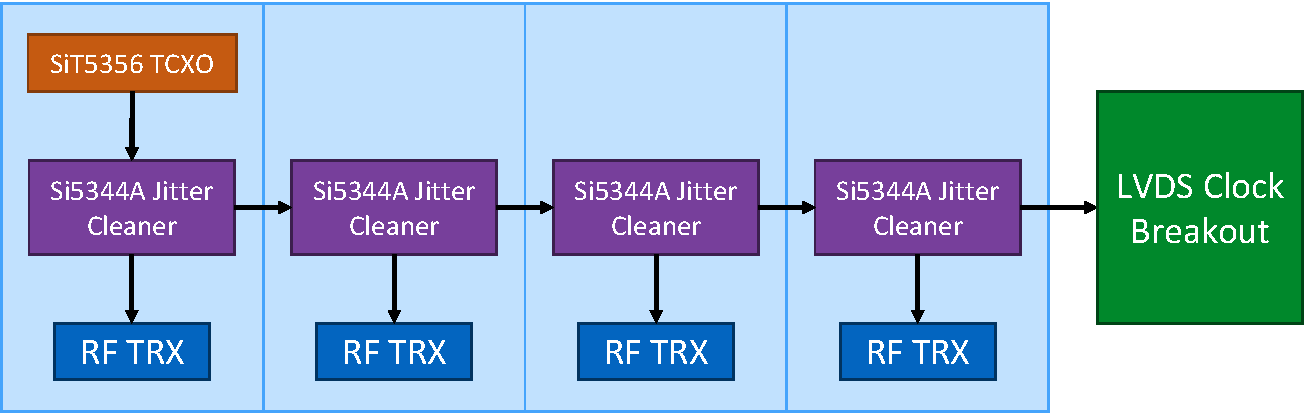
\includegraphics[width=0.9\textwidth]{figs/clk/iris030_diagram}
\caption{Block diagram of IRIS-030 jitter cleaned daisy chain clocks.}
\label{fig_030_chain}
\end{figure}
	
	The improved design goal for the IRIS-030 system shown in Figure~\ref{fig_iris_pictures} (right) was to achieve a forwarded clock phase jitter less than 1.5~ps RMS given system design parameters of 80~MHz modulation bandwidth and \ac{ADC} resolution of 10 bits \cite{brannon2006jitter}.
	This \ac{SDR} module utilizes a daisy-chained clock jitter cleaner at each intermediate node in order to filter clock phase noise at each step and re-synthesize RF and baseband reference clocks from the cleaned clock and forward to the next node (Figure~\ref{fig_030_chain}).
	
	Based on these specifications, we chose to use a temperature-controlled MEMS oscillator for the IRIS-020 with a specification of 1.7~ps \ac{RMS} period jitter and a clock buffer IC with a specification of 0.02~ps additive phase jitter to minimize additive jitter from forwarded steps.
	The IRIS-030 received an improved specification of 0.8 \ac{RMS} period jitter to match the more stringent specifications for the later design.
	
	The clock jitter cleaner topology and general clocking diagram for the IRIS-030 is presented in Figure~\ref{fig_030_clk_diagram}.
Upstream clocks are filtered through a high-performance \ac{PLL} and digitally-controlled frequency synthesizer, Si5344, which generates low-jitter reference clocks for the high-speed serializer circuits, \ac{DAC}/\ac{ADC} blocks, and RF frequency synthesizers.

We tested the clocking jitter using the jitter measurement feature of a Keysight DSO8040B 40 GSa/s oscilloscope and three operational IRIS-020 prototypes with daisy-chained clocks, comparing their results to that of a set of four daisy-chained IRIS-030 modules with jitter-cleaned clocks.
Figure~\ref{fig_iris_pictures} shows the implemented radio clock chain hardware, representing a 6-radio \ac{MIMO} cluster (left) and an 8-radio \ac{MIMO} cluster (right).

% Iris Clocking Diagram with Jitter Cleaning
\begin{figure}[p]
\centering
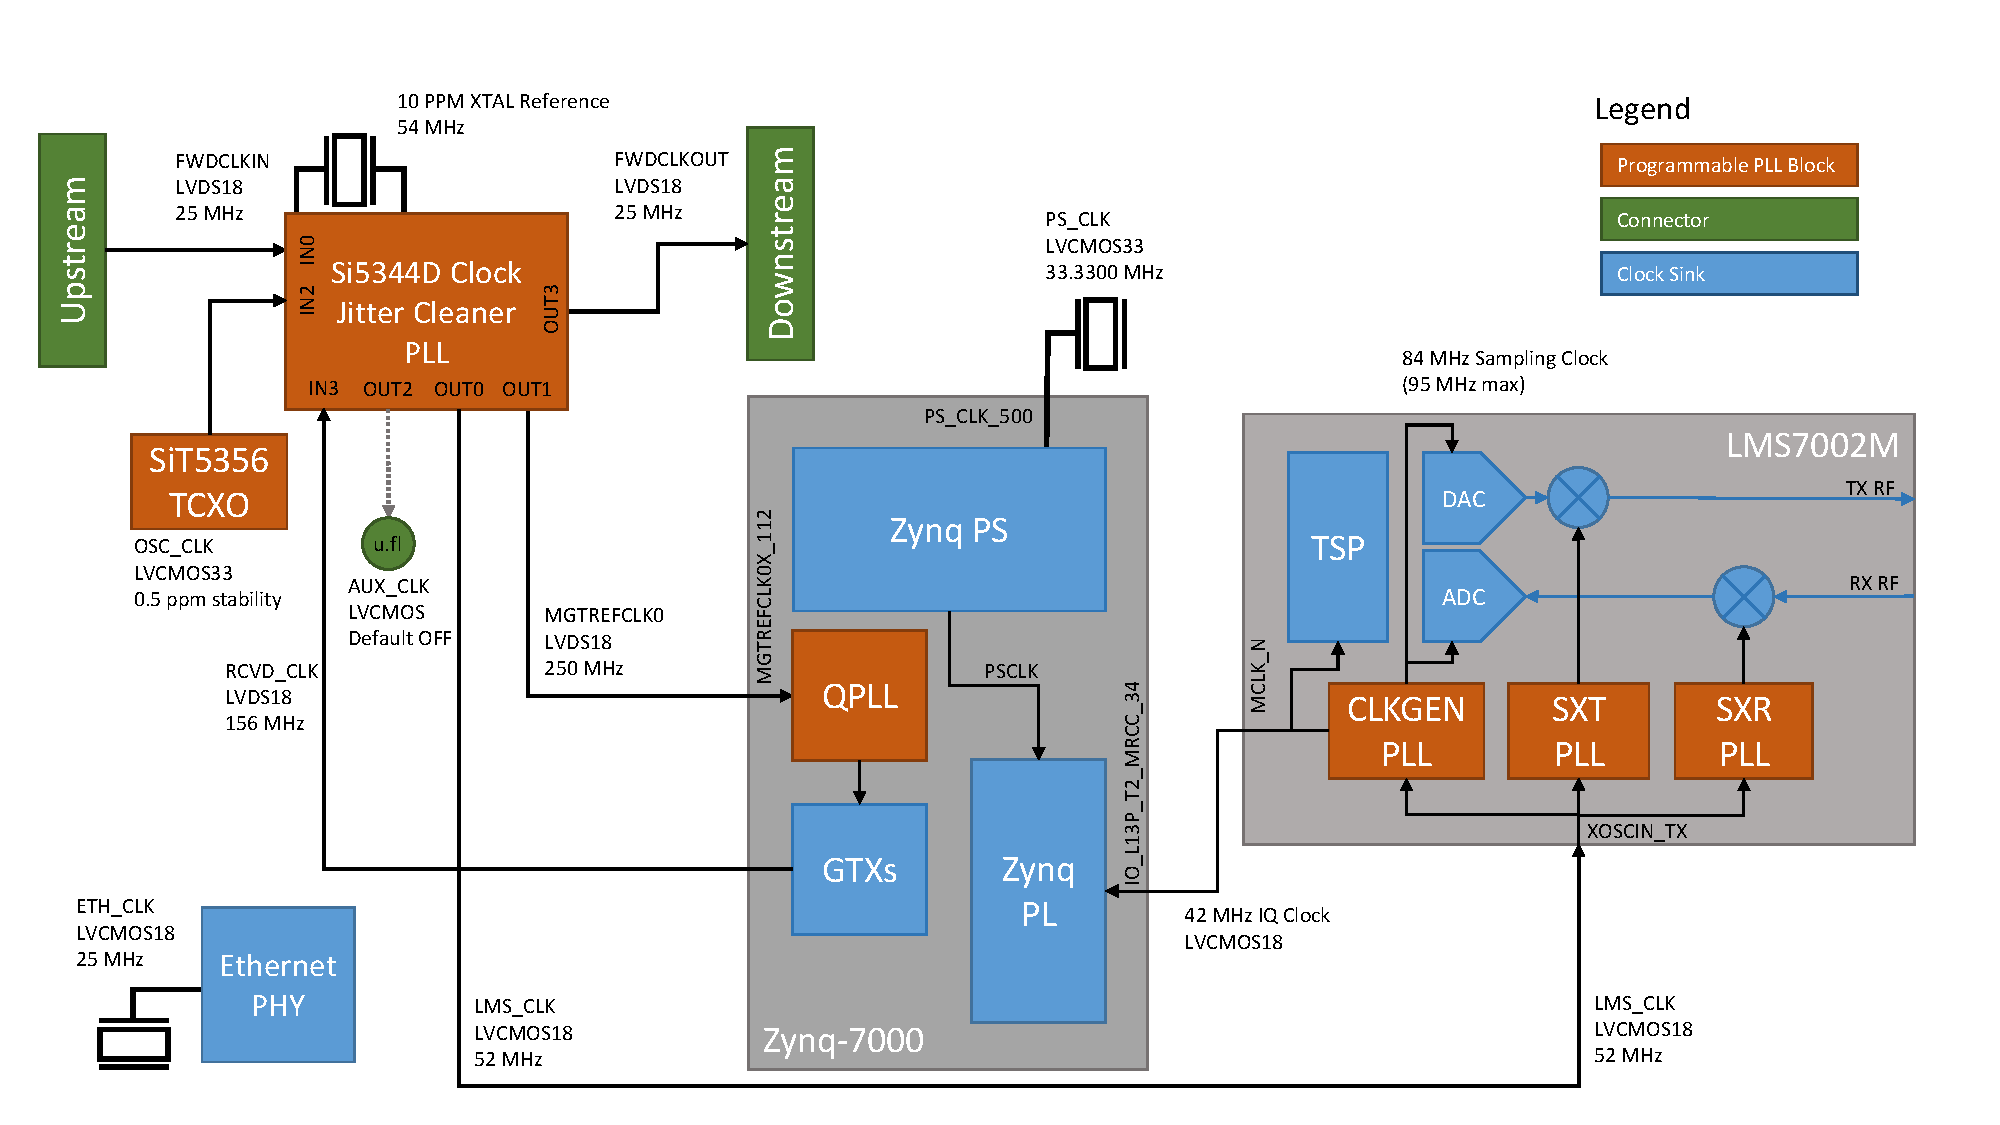
\includegraphics[width=1\textwidth]{figs/clk/iris_clocking_diagram}
\caption{Diagram of IRIS-030 clocking system with jitter cleaner.}
\label{fig_030_clk_diagram}
\end{figure}



% Daisy Chain Clocking Setup
\begin{figure}[p]
\centering
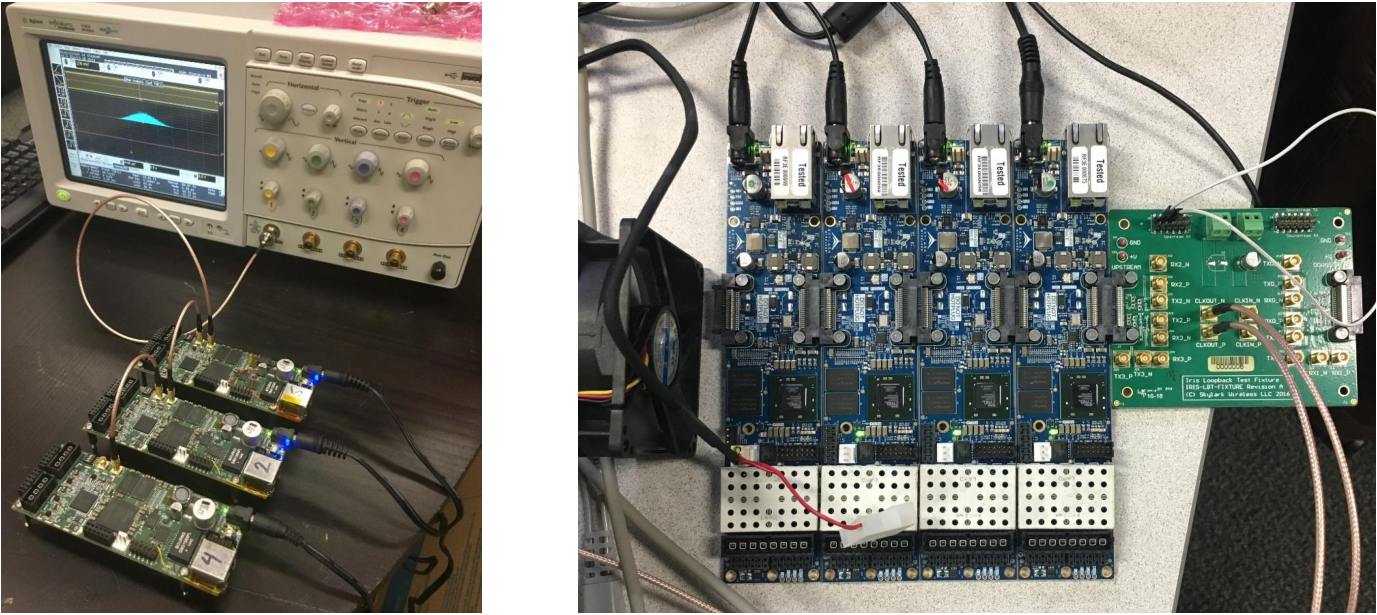
\includegraphics[width=1\textwidth]{figs/clk/iris020_iris030_pics}
\caption{Test setup for IRIS-020 (left) and IRIS-030 (right) clocking measurements.}
\label{fig_iris_pictures}
\end{figure}

% Buffered vs. Cleaned Jitter Performance
\begin{figure}[p]
\centering
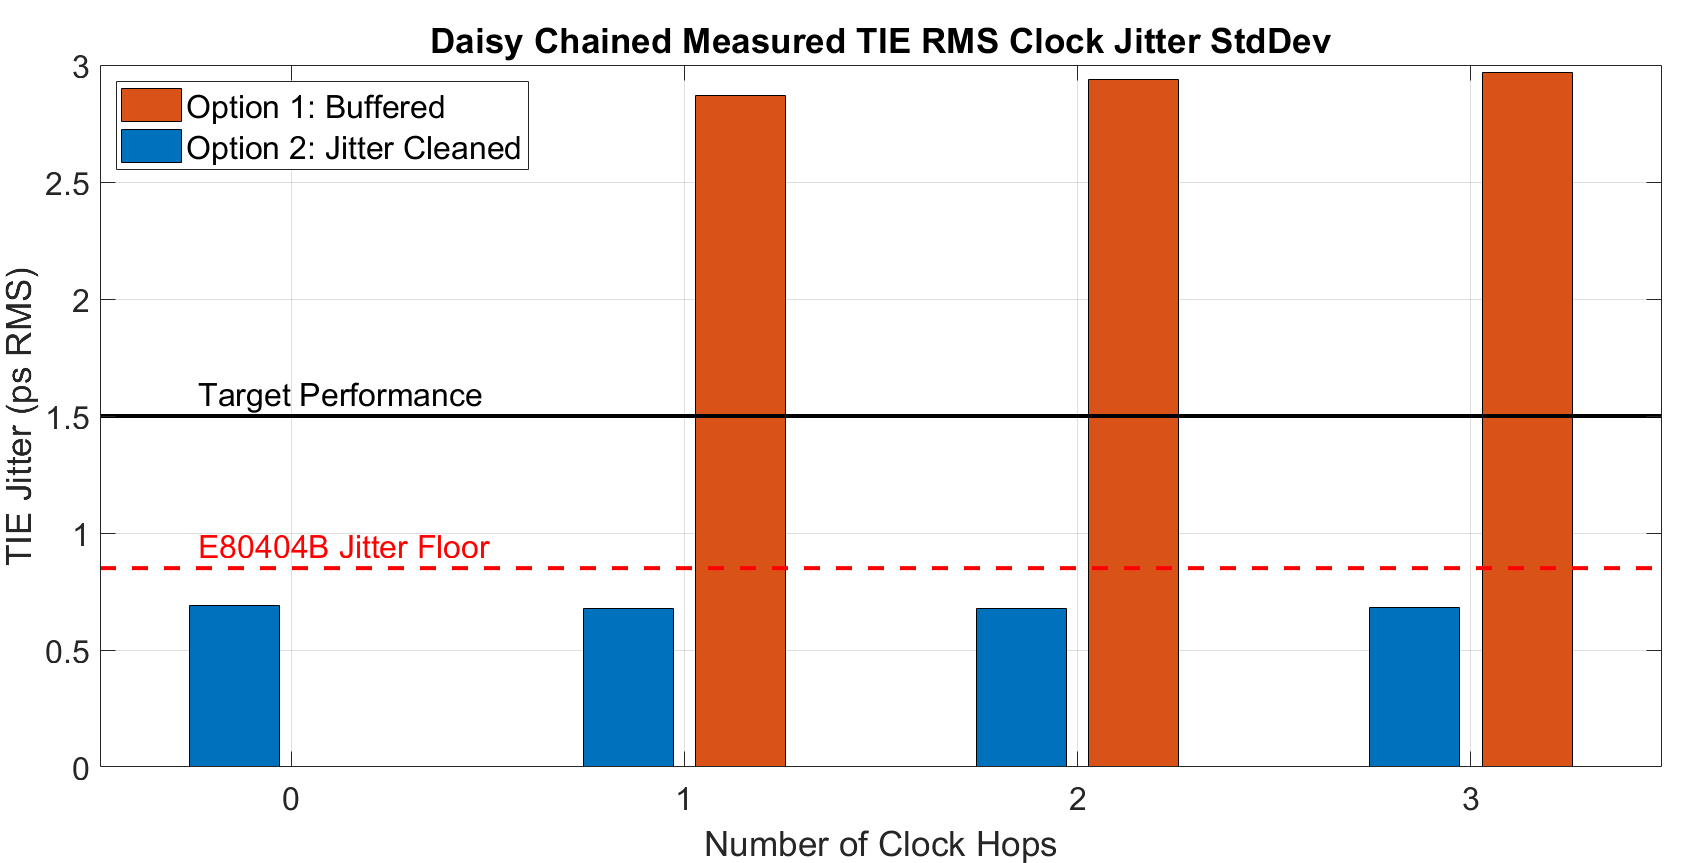
\includegraphics[width=1\textwidth]{figs/clk/iris_jitter_barplot}
\caption{Measured clock RMS TIE jitter as a function of the number of daisy-chain hops for both IRIS-020 (buffered) and IRIS-030 (jitter cleaned) daisy-chains.}
\label{fig_multihop_jitter}
\end{figure}

	At the time of the measurement, only three prototype IRIS-020 units were available for characterization.
	Furthermore, the equipment available at the time could not directly measure phase jitter noise spectra; instead we chose to measure RMS Time Interval Error (TIE), which is loosely equivalent, yet on a different measurement scale \cite{an687}.
	Forwarded output clock jitter measurements were made from over 10,000 recorded clock transitions at each output stage of the clocking daisy chain.
	We compared the buffered clock forwarding on the IRIS-020 module with that of the jitter-cleaned clock forwarding on the IRIS-030.
	The recorded measurements in Figure~\ref{fig_multihop_jitter} are given in picoseconds of RMS time-interval jitter. The targeted 1.5~ps RMS TIE jitter target is given as the black solid line.
	The DSO80404B has a 0.85 ps rms TIE jitter measurement floor shown as the red dotted line.
	
	For the buffered clock forwarding scheme, we observed a maximum of 0.07 ps additive TIE jitter for each additional daisy chained IRIS-020 module, which is consistent with our target specifications, but which provides little margin for additional chain length.
	In addition, we found that the orientation and order of modules impacted our measurements significantly, since the output buffer jitter proved to be very sensitive to the cable connections for input and output clocking within the daisy-chain.
	In the middle of the chain, any weak connection or poor cable would decrease the quality of the clock for the rest of the downstream chain significantly.
	The results presented in Figure~\ref{fig_multihop_jitter} are the best-case measurements out of the set of data observed in order to best represent the buffered clock topology rather than any particular physical implementation of it.
	
	This issue of noisy channels for forwarded clocks on the IRIS-020 was addressed in the later IRIS-030 design by the use of direct-attach connectors without cabling as well as the use of differential clock signaling, which proves to be more robust to common-mode noise.
	In addition, the clock jitter cleaner topology shown in Figure~\ref{fig_030_clk_diagram} provides the ability to filter jitter from the clocking signal at each step as it moves down the daisy-chain.


% Iris Jitter Cleaned Clock
\begin{figure}[p]
\centering
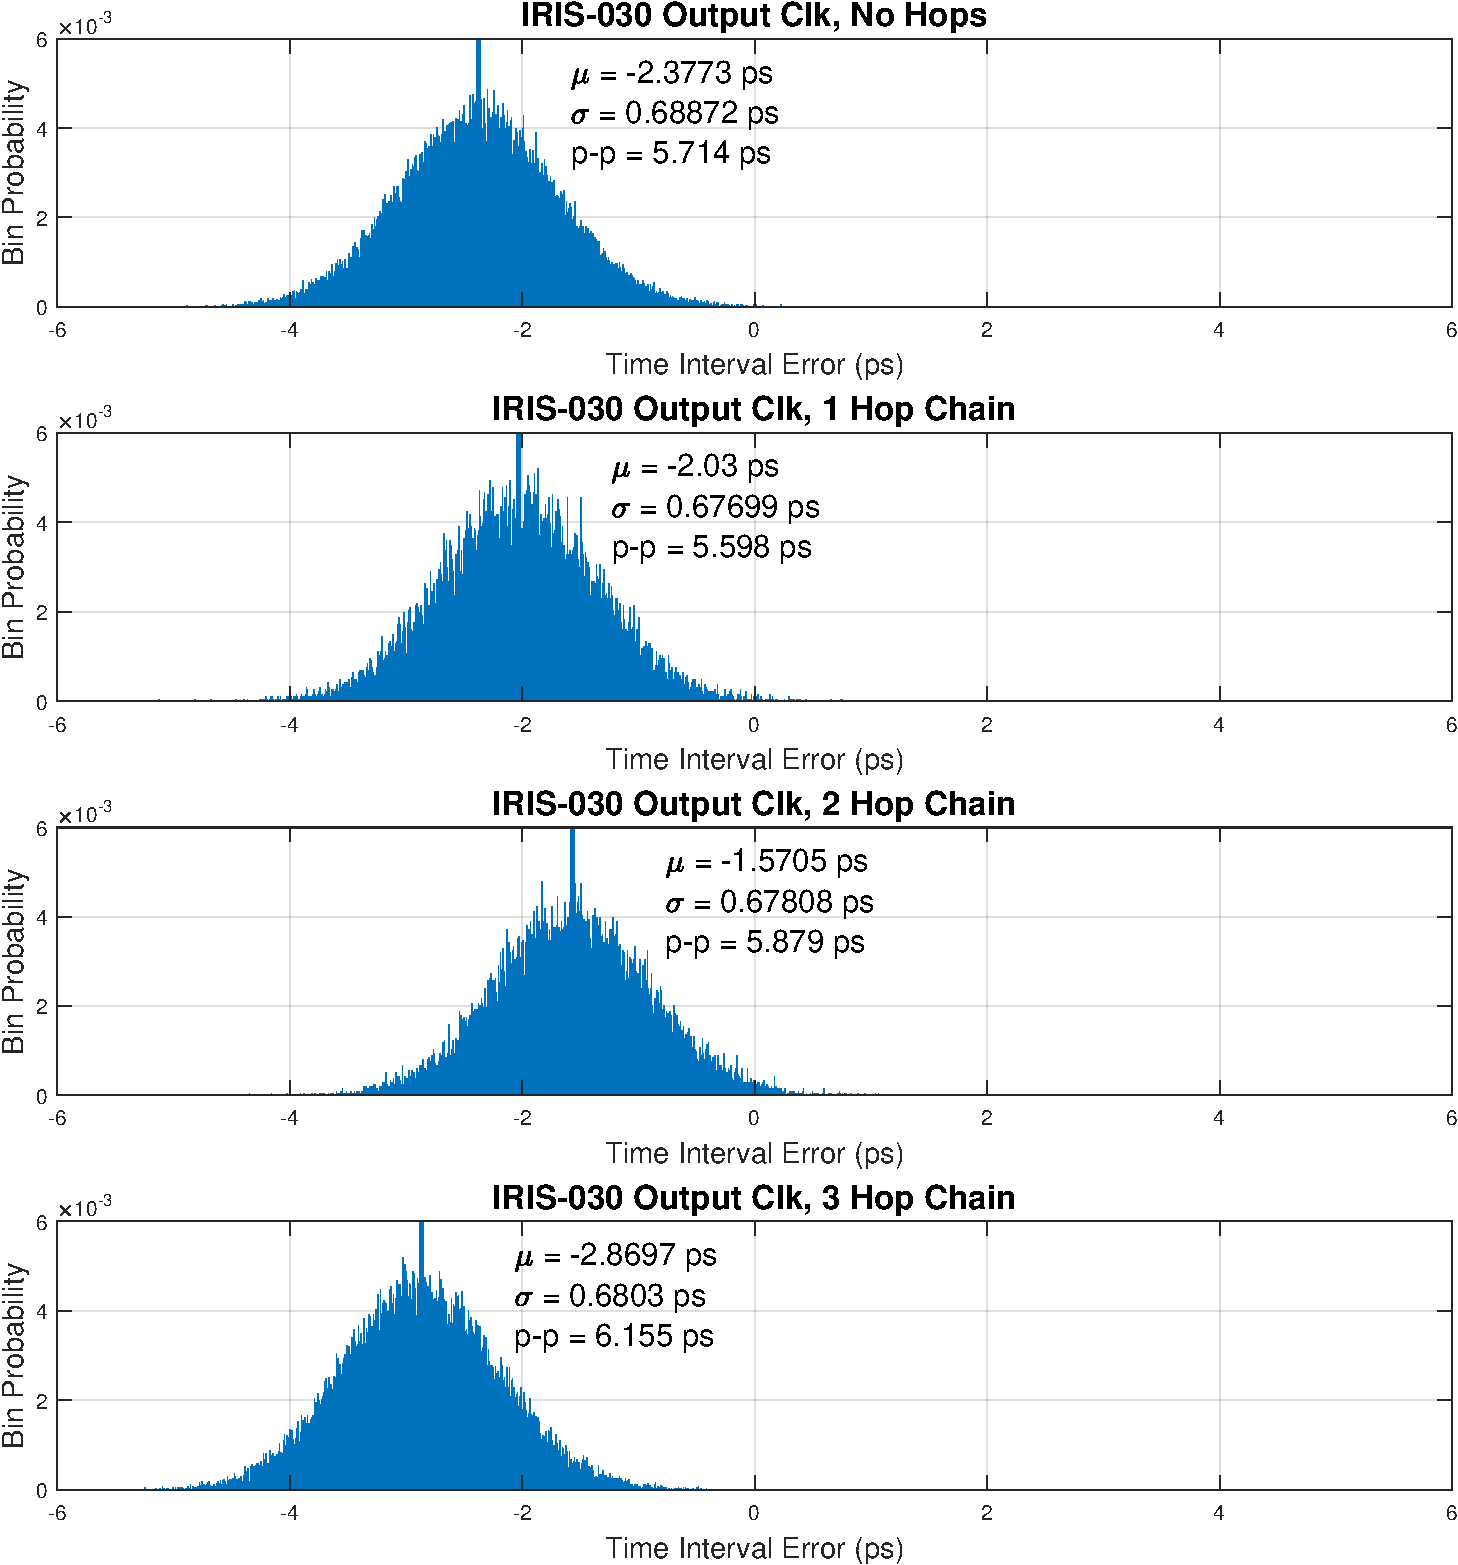
\includegraphics[width=1\textwidth]{figs/clk/iris030_multihop_jitter}
\caption{IRIS-030 reference clock jitter as a function of daisy chain hops.}
\label{fig_030_clk_jitter}
\end{figure}


In Figure~\ref{fig_030_clk_jitter} we show the measured \ac{RMS} \ac{TIE} jitter \ac{PDF} for each hop of the IRIS-030 chain shown in Figure~\ref{fig_iris_pictures} (right).
We find that the noise \ac{PDF} does appear to be Gaussian, with a mean relative to the measurement time base that is arbitrary, indicating that the forwarded clocks are, in fact, syntonized, with similar jitter distributions at the output of the clock jitter cleaners. 

This experimental setup was repeated with a longer chain of 10x IRIS-030 modules shown in Figure~\ref{fig_10x_hop_setup} with similar findings: for up to 10x daisy-chain hops, the successive clock jitter cleaning stages keep reference clock jitter well below the threshold for measurement with the test equipment used.
The use of 1.8~V \ac{LVDS} for clock forwarding provided additional systemic noise immunity.

% Jitter comparisons of various hardware and IOs.
\begin{figure}[h]
\centering
  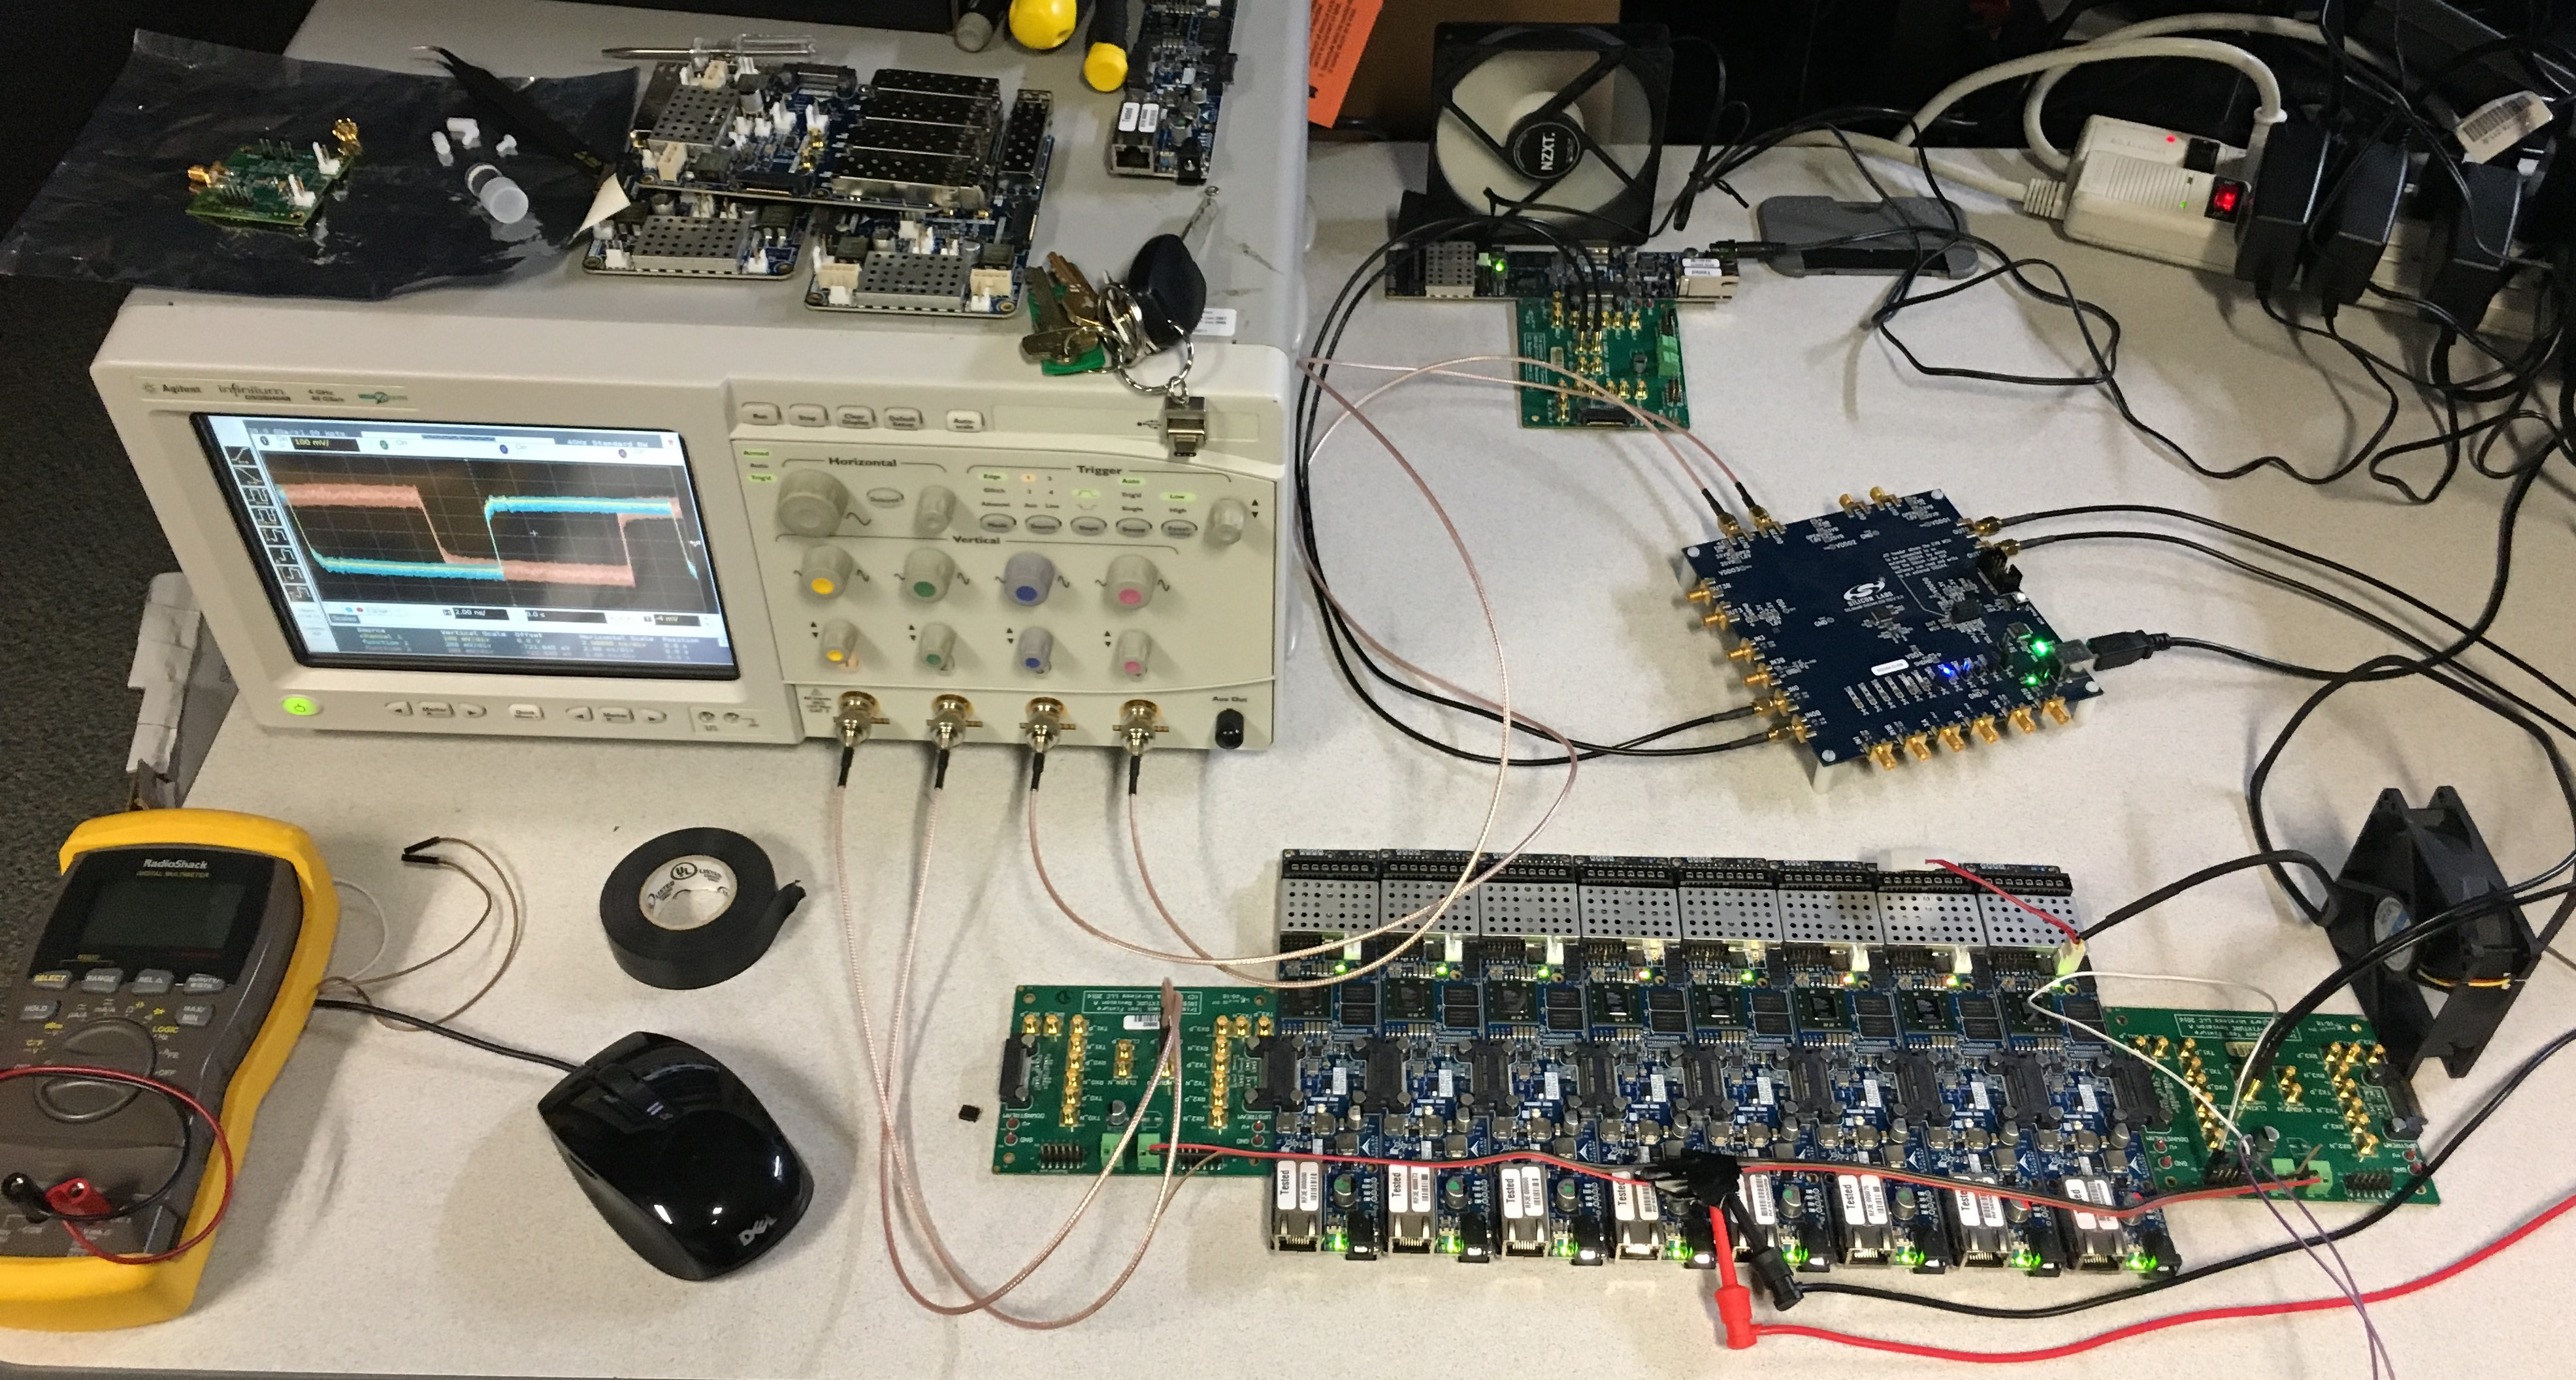
\includegraphics[width=1\linewidth]{figs/clk/030_clocking_chain}   
    \caption{Test setup with 10x daisy-chained IRIS-030 modules with Si5344 development board on the second hop.}
\label{fig_10x_hop_setup}
\end{figure}


% Jitter comparisons of various hardware and IOs.
\begin{figure}[h]
\centering
  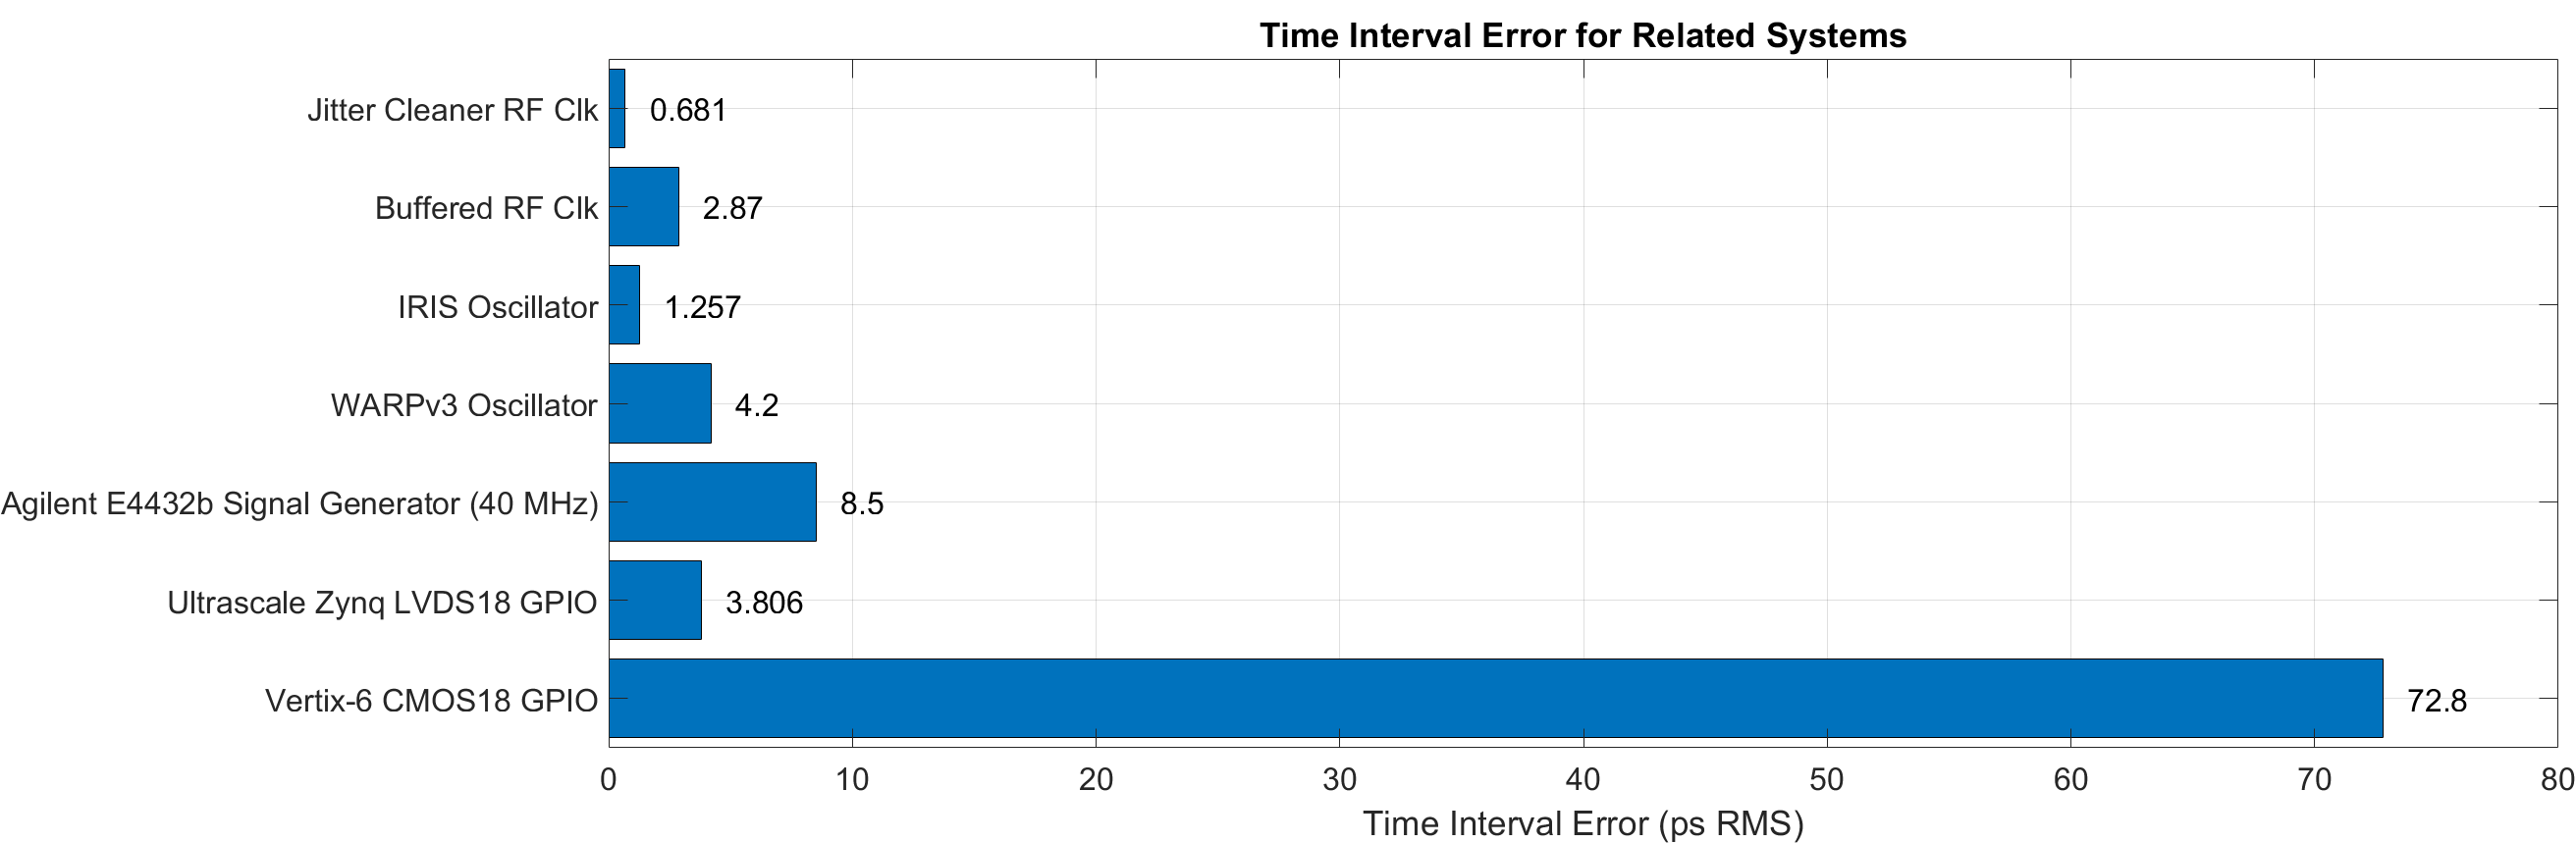
\includegraphics[width=1\linewidth]{figs/clk/iris_jitter_common_things}   
    \caption{Experimental comparison of \ac{RMS} \ac{TIE} jitter for various clock sources and \ac{FPGA} I/O standards.}
\label{fig_jitter_comparisons}
\end{figure}

Although provided in vendor specification sheets, we took the extra step of comparing the reference clock jitter of clocking outputs of the various generations of equipment used in our test setups and show the resulting \ac{RMS} \ac{TIE} jitter measurements in Figure~\ref{fig_jitter_comparisons}.

Based on our measurements, the noise on the output of the jitter cleaner on the IRIS-030 has the lowest \ac{TIE} value, with the source SiT5256 (``IRIS Oscillator'') reference a close second.
The buffered reference clock sourced from an SiT5000 oscillator on the IRIS-020 module has slightly better performance than the original WARPv3 reference hardware, which we can attribute to the method of directly probing the oscillator pads on the WARPv3 hardware with a single-ended probe while we used a coaxial cable to measure the IRIS-020 reference clock.
This reference derived from the SiT5000 has just about the same performance as a modern-day \ac{LVDS} output from an UltraScale Zynq, whereas the WARPv3 Vertix-6 CMOS I/O architecture has extremely high clocking noise.

In conclusion, we empirically demonstrate that the coherent clock distribution system behaves as designed in-situ across various platforms, and provide a direct comparison allowing the future system designer to trade cost (jitter cleaner hardware is expensive in both energy and price) against RF performance (maximum modulation bandwidth supported by system clock jitter) in future designs.


%###############################################
\subsection{Distributed Multi-Hop Clock Synchronization}
\label{sec_clk_sfp}

In this final section, we put the pieces together to implement and test a distributed, coherent \ac{MIMO} RF clock distribution network using the recovered clocks from fiber channel links in order to provide syntonicity to physically separate radio clusters.
In this design, we use a 64B/66B encoder/decoder pair to embed and recover the serial clock reference implicitly included in a high-speed serial link \cite{toyoda2010100gbe}.
The 64B/66B encoder ensures that level transitions are always present in the serial data stream, thus enabling Xilinx \ac{PHY} transceiver primitives to recover and export the reference clock, which remains syntonized to the input serial stream.
On Synchronous Ethernet systems such as the Arista 7150S SFP+ switch hardware used in our evaluation, the source serial transmitters share reference clocks across data ports, meaning that all serial receivers will also be synchronized \cite{rec2007g}.

Our contribution is to recognize the relatively poor jitter performance of the recovered serial reference clock (Figure~\ref{fig_jitter_comparisons}, ``Ultrascape Zynq LVDS18 GPIO'') and to route that clock through the on-board clock jitter cleaner in the IRIS-030 architecture in order to create a syntonized, low-jitter RF reference.
Since the clock is distributed over fiber channel links, the source and destination syntonized nodes may be as much as 10~km apart based on the maximum distance of commodity fiber channel single-mode laser transceivers.

We provide the complete design for distributed, modular, and frequency-agile \ac{SDR} systems that can be rapidly re-configured in any of a number of different configurations.

We first test this system implementation and the ability of a recovered fiber-channel serial clock to maintain syntonicity over a long period of time by implementing the prototype design in Figure~\ref{fig_zcu_diagram_pic} utilizing two different GTH serial transceiver channels operating on independent transceiver ``tiles'' on a Xilinx ZCU102 \ac{FPGA} development board.
Two 10~Gbps fiber channel links with synchronous source clock references from the switch are recovered and exported independently to a Keysight DSO8040B oscilloscope for analysis.

We then repeat this test using production IRIS-030 serial transceiver hardware and the built-in Xilinx GTX serial transceivers using two separate \ac{SDR} modules and observe the same performance, proving that syntonicity was not an artifact of the single \ac{FPGA} architecture or the prototype ZCU102 project.

% ZCU102 Clocking Diagram
\begin{figure}[p]
\centering
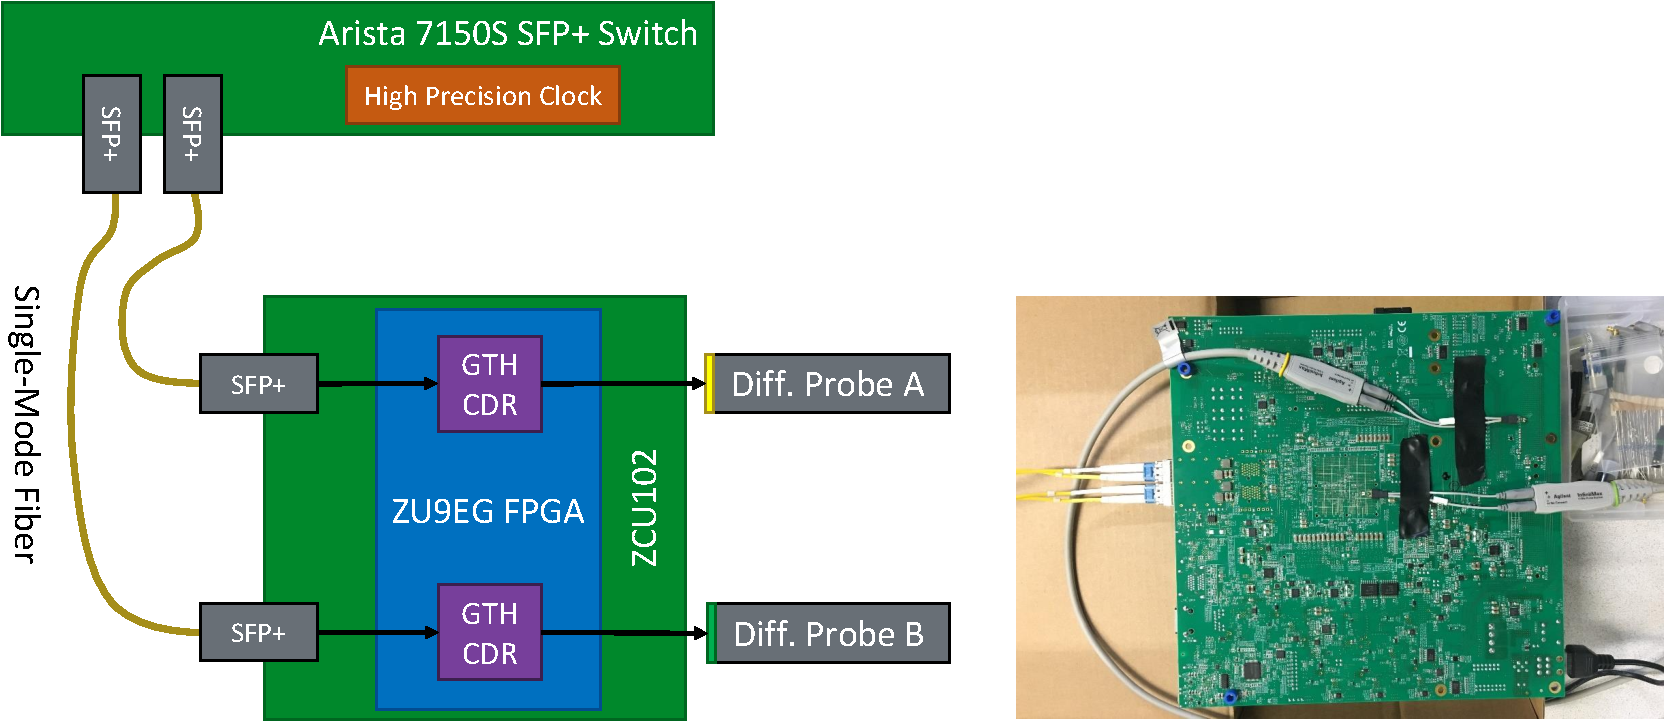
\includegraphics[width=1\textwidth]{figs/clk/zcu102_clocking_diagram}
\caption{Diagram of distributed clocking structure prototype on Avnet ZCU102 board.}
\label{fig_zcu_diagram_pic}
\end{figure}

% IRIS-SFP Clocking Diagram
\begin{figure}[p]
\centering
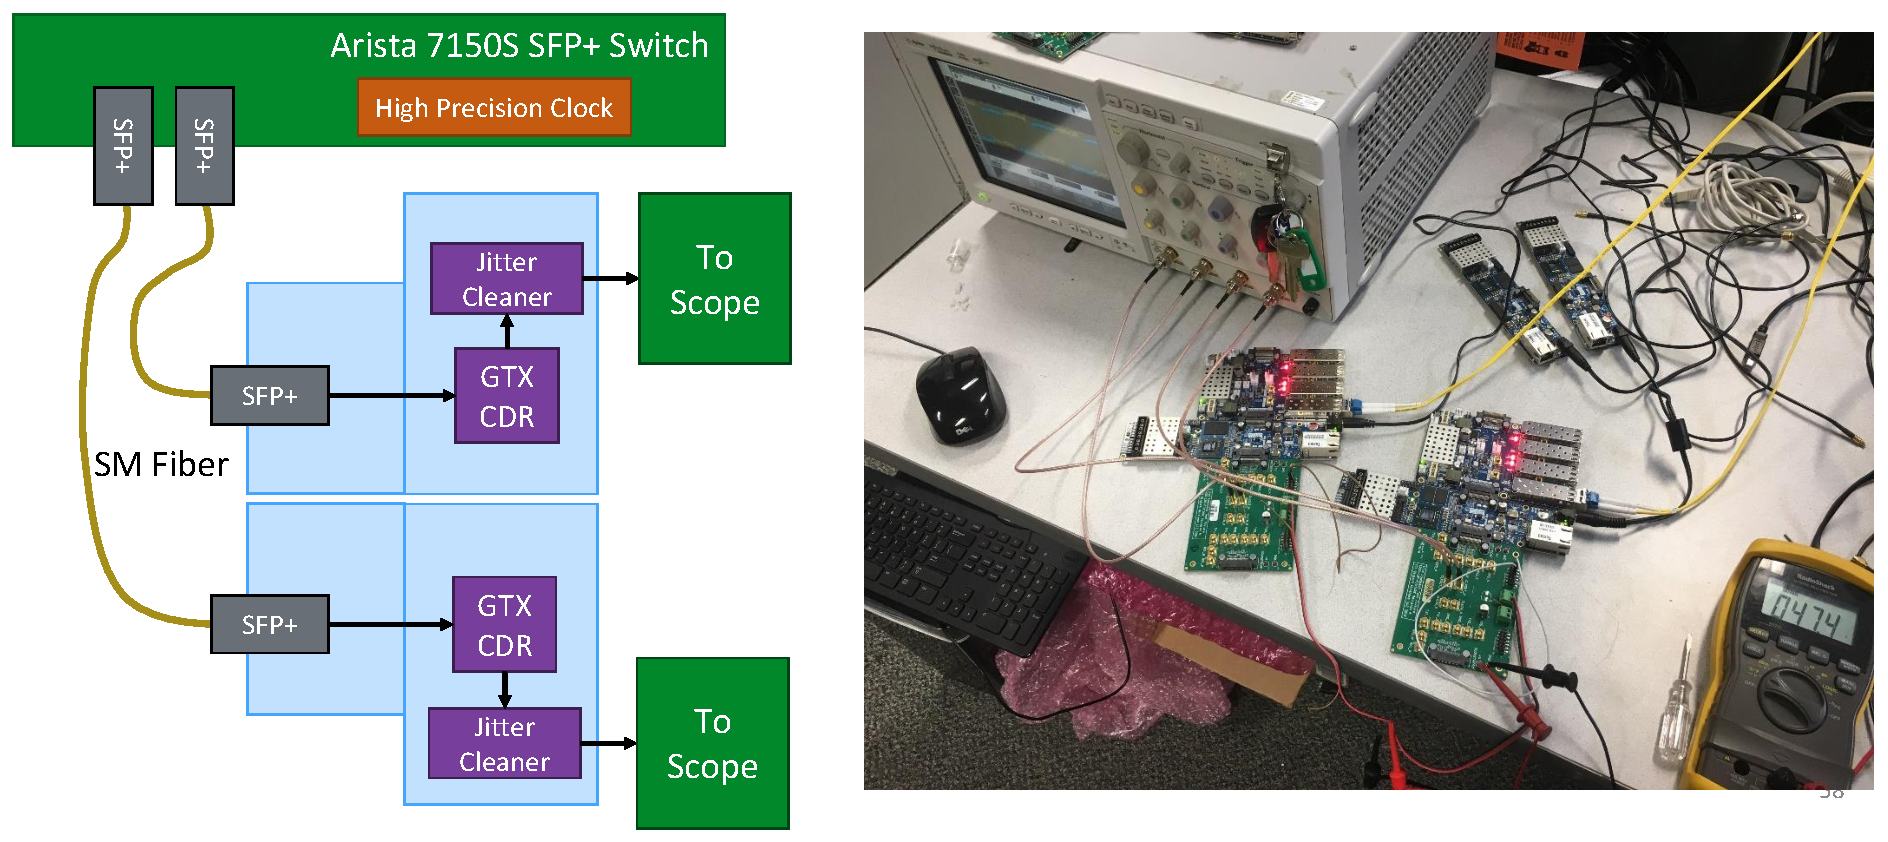
\includegraphics[width=1\textwidth]{figs/clk/sfp_clock_diagram}
\caption{Diagram of distributed clocking structure on production IRIS-030 equipment.}
\label{fig_sfp_diagram}
\end{figure}

The recovered and exported clocks directly exported by the 1.8~V \ac{FPGA} \ac{LVDS} were observed to have the \ac{RMS} \ac{TIE} jitter as shown in Figure~\ref{fig_030_clk_jitter}, with the standard deviation of approximately 3.8~ps.
While this clock exceeds the 1.5~ps limit to be used as an RF reference for an 80~MHz modulation bandwidth converter with 10 bits, we are abe to demonstrate that these reference clocks are long-term syntonized by displaying a persistent plot of the two RF reference clocks in both systems with (right) and without (left) reference fiber channel locks in Figure~\ref{fig_zcu_lock}.

In both cases, the system is left to run over 24 hours, triggering constantly on the clock A (yellow). When clock A and B are syntonized, the relative phase between A and B should remain locked.
In the left image, without fiber channel lock, clock B is constantly sweeping all relative phase positions to clock A, resulting in the uniform green grayed out region in the persistent oscilloscope display.
In the right image with a fiber channel lock, clock B is consistently phase locked (or syntonous) to clock A over the course of 24 hours and never changes its phase relationship.


% ZCU102 Recovered Clock Jitter
\begin{figure}[p]
\centering
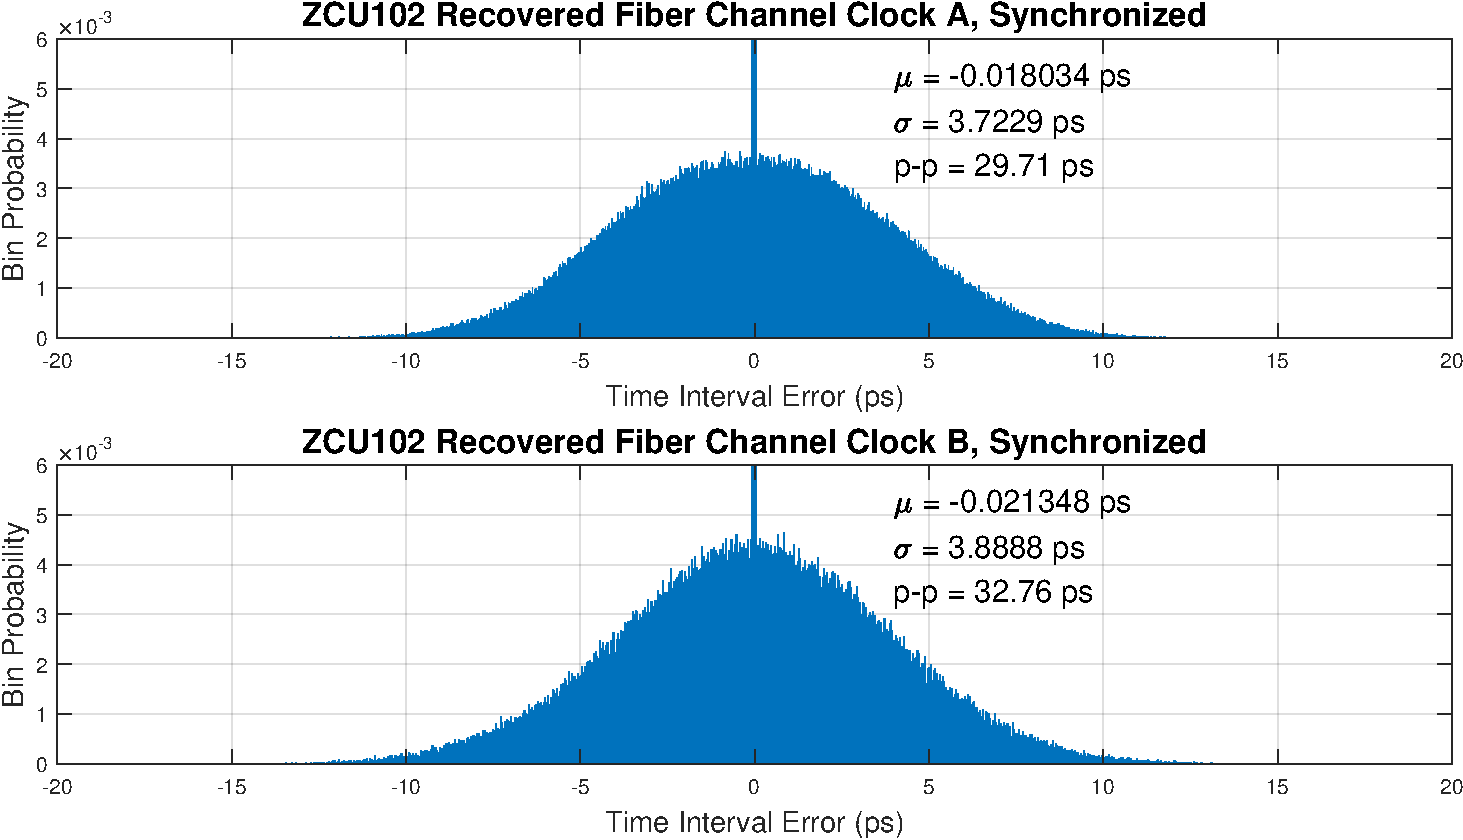
\includegraphics[width=1\textwidth]{figs/clk/zcu102_recovered_jitter}
\caption{Fiber channel recovered clock jitter for ZCU102 FPGA board.}
\label{fig_030_clk_jitter}
\end{figure}

% Clock Lock Experiment
\begin{figure}[p]
\centering
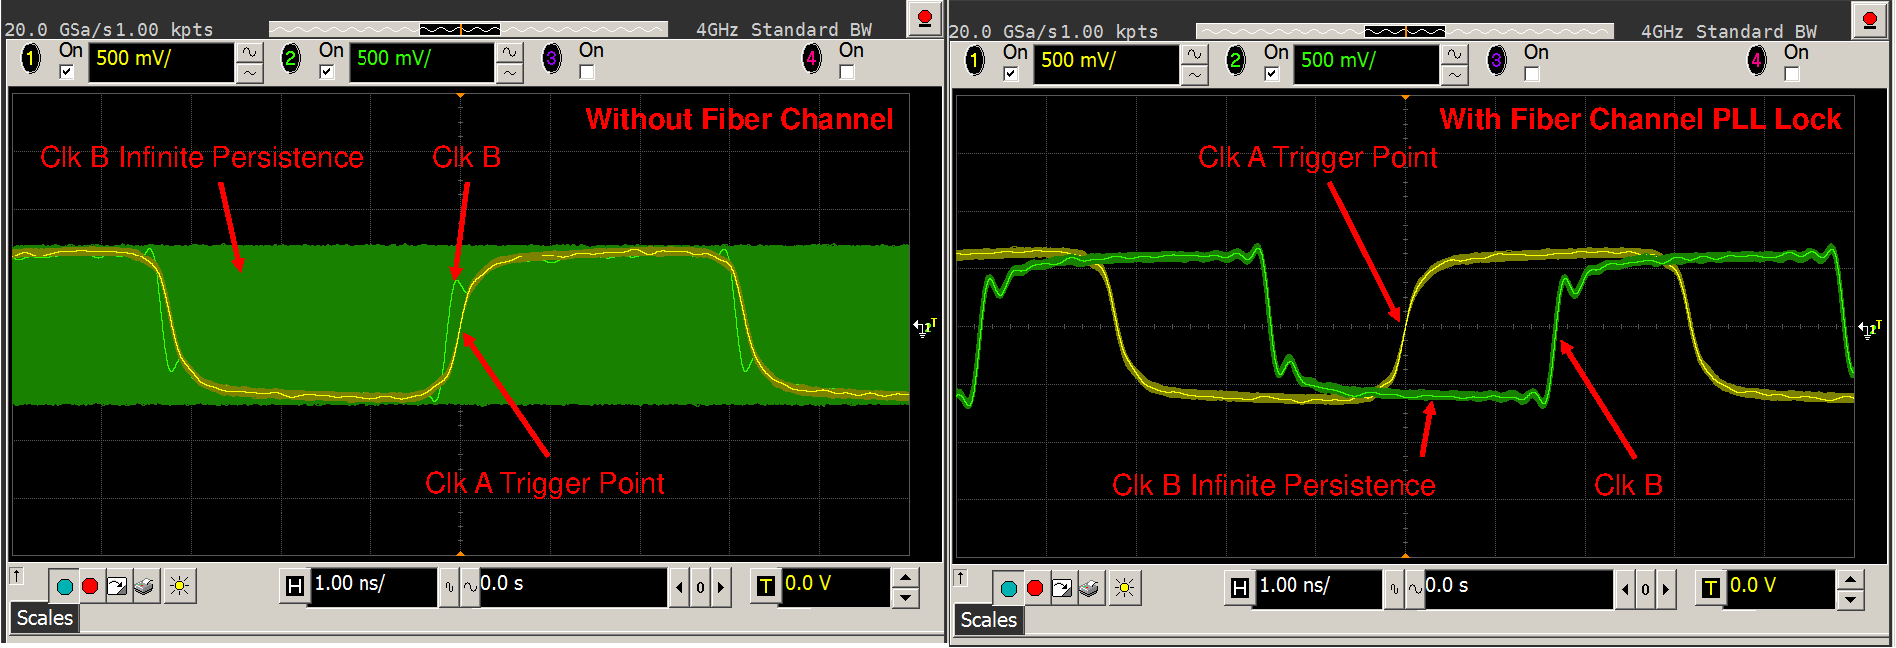
\includegraphics[width=1\textwidth]{figs/clk/zcu102_clock_lock}
\caption{24-hour clock phase lock results for ZCU102 setup.}
\label{fig_zcu_lock}
\end{figure}

These system validations, when combined with the daisy-chain clocking topology presented in Section~\ref{sec_daisy_chain_clocking}, allow us to create arbitrarily-sized radio daisy-chains using IRIS-030 hardware and distribute them over a large geographical area.

In practice, this is important when distributing radios and antennas in an arbitrarily-large \ac{TVWS} array where the spatial separation of antennas may be on the order of a half-meter.
Having the flexibility to configure any number of radios in any position and maintain RF coherency is a key benefit of our modular clocking design.

\pagebreak
